
% Copyright 2020 by Robert Hildebrand
%This work is licensed under a
%Creative Commons Attribution-ShareAlike 4.0 International License (CC BY-SA 4.0)
%See http://creativecommons.org/licenses/by-sa/4.0/

%\documentclass[../open-optimization/open-optimization.tex]{subfiles}
%\newcommand{\floor}[1]{\lfloor #1 \rfloor}
%\newcommand{\ceil}[1]{\lceil #1 \rceil}
%
%\renewcommand{\intr}{\mathrm{int}}
%\usepackage[many]{tcolorbox}
%
%\tcbuselibrary{skins,breakable, theorems}
%\usepackage{changepage}% for use of \ifoddpage below
%
%\newtcbtheorem[number within=chapter]{mytheorem}{Theorem}%
%{colback=yellow!5,colframe=yellow!35!brown,fonttitle=\bfseries}{th}
%
%
%\newtcbtheorem[number within=chapter]{mydefinition}{Definition}%
%{colback=blue!5,colframe=blue!35!black,fonttitle=\bfseries}{th}
%
%%\tcbset{
%%  theorem style/theorem wide name and number/.code={ \let\tcb@theo@title=\tcb@theo@widetitle},
%%  proofbox/.style={skin=enhancedmiddle,breakable,parbox=false,boxrule=0mm,
%%    check odd page, toggle left and right, colframe=thmLnColor,
%%    leftrule=8pt, rightrule=0mm, boxsep=0mm,arc=0mm, outer arc=0mm,
%%    left=3mm,right=0mm,top=0mm,bottom=0mm, toptitle=0mm,
%%    bottomtitle=0mm,colback=white,
%%    before={\par\vskip-2pt},after={\par\smallbreak},
%%  },
%%}
%\tcbset{
%  proofbox/.style={breakable},
%}
%\newtcolorbox{ProofBox}{proofbox}
%
%\let\realproof\proof
%\let\realendproof\endproof
%\renewenvironment{proof}{\ProofBox\textbf{Proof.  }}{\hfill \qedsymbol \endProofBox}
%
%
%\begin{document}

\chapter{Cutting Planes}
\section{Introduction}

\subsection{Cutting planes}
 \index{Cutting Planes}
\begin{definition}{Cutting plane for IP}{IP-cuts} Let $P\subseteq\R^n$ be a polyhedron. An inequality $a^Tx\leq b$ is called a \emph{cutting plane }if 
$$P\cap\Z^n\subseteq \{x\in\R^n\tq a^Tx\leq b\}.$$
\end{definition}

\begin{definition}{Cutting plane for MIP}{MIP-cuts} Let $P\subseteq\R^n$ be a polyhedron. An inequality $a^Tx\leq b$ is called a \emph{cutting plane} if 
$$P\cap(\Z^{n_1}\times\R^{n_2} ) \subseteq \{x\in\R^n\tq a^Tx\leq b\},$$
where we are assuming that in the MIP only the first $n_1$ variables must be integers ($n=n_1+n_2$).
\end{definition}

\subsection{Cutting plane algorithm}

\begin{multicols}{2}

{\bf Generic cutting plane algorithm}

\vspace{-1cm}

\begin{enumerate}
\setlength{\itemsep}{0.01cm}
\item {\bf  Solve} LP (continuous relaxation of MILP).
\item If solution of LP is {\bf  fractional}: add cutting plane and go to (1.)
\item If solution of LP is {\bf integral}: { \bf STOP}.
\end{enumerate}

\columnbreak

\begin{center}
%\begin{figure}%
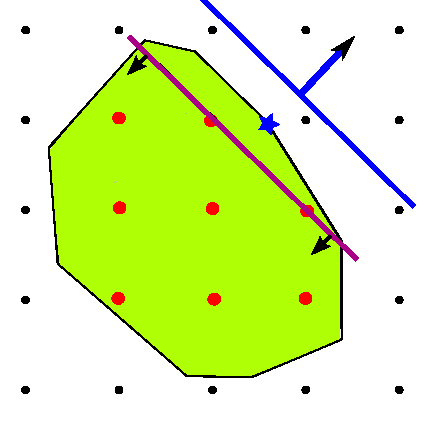
\includegraphics[scale=0.75]{CPalgorithm6.pdf}
%\end{figure}
\end{center}

\end{multicols}

\vspace{-1cm}

\subsection{How to compute cutting planes}

Two approaches:

\begin{enumerate}
	\item Computing cutting planes for general IPs.
	\begin{itemize}
		\item From ``Algebraic'' properties: CG cuts, MIR inequalities, functional cuts, etc.
		\item From ``Geometric'' properties: lattice-free cuts, etc.
	\end{itemize}
	
		\item Computing cutting planes for specific IPs.
	\begin{itemize}
		\item Knapsack problem, Node packing, etc. (many many other examples\dots)
	\end{itemize}
\end{enumerate}

\subsection{Cutting planes from the Simplex tableau}
Assume $P=\{x\in\R^n\tq Ax=b,\ x\geq0\}$ where $A\in\R^{m\times n}$ is a full-row rank matrix. Let $B$,$N$ denote the basic and nonbasic variables defining a vertex $(\hat x_B,\hat x_N)$ of $P$ (where $\hat x_N=0$). You can write the constraints defining $P$ in terms of the basis $B$:
\begin{align*}
x_B&=\bar b -\bar A_N x_N\\
&x_B,x_N\geq0,
\end{align*}
where $\bar b=A_B^{-1}b$ and $\bar A_N=A_B^{-1}A_N$. 

\vspace{0.2cm}

Denote $\bar b=(\bar b_i)_{i\in B}$ and  $\bar A_N=(\bar a_{ij})_{i\in B, j\in N}$. Assume that $\bar b_i\notin \Z$, so the vertex is fractional \big(that is, $(\hat x_B,\hat x_N)\notin \in \Z^n$\big), and therefore, we would want to cut off that LP solution.

\begin{remark}{}{} Recall that the vertex $(\hat x_B,\hat x_N)$ is the only feasible point in $P$ satisfying $x_N=0$. We will use this fact in order to derive some cutting planes.
%\begin{align*}
%x_B&=\bar b \\
%x_N&=0.
%\end{align*}
%We will use this fact in order to derive some cutting planes.
\end{remark}

\subsubsection{Gomory's fractional cut}
Suppose we have $x \in \Z^n_+$ with $x_i \in \Z$, along with the equation
\begin{equation}
\sum_{i \in I} a_{i}x_{i} = b.
\end{equation}
Then the following inequality can be derived as a Chvatal cut:
\begin{equation}\sum_{j\in N}\big(\bar a_{ij}-\lfloor \bar a_{ij} \rfloor \big)x_j\geq (\bar b_{i}-\lfloor \bar b_{i} \rfloor \big).\end{equation}

Let $f = \bar b_{i}-\lfloor \bar b_{i} \rfloor $.  Then this can be equivalently written as 

\begin{equation}\sum_{j\in N}\left( \frac{\bar a_{ij}-\lfloor \bar a_{ij} \rfloor}{f}\right) x_j\geq 1.\end{equation}



It can be verified that this valid inequality cuts off the fractional vertex.

\begin{figure}[h]
\begin{tikzpicture}
    \begin{axis}[
        axis x line=middle,
        axis y line=middle,
        grid = major,
        width=8cm,
        height=8cm,
        grid style={dashed, gray!30},
        xmin=0,     % start the diagram at this x-coordinate
        xmax= 1,    % end   the diagram at this x-coordinate
        ymin= 0,     % start the diagram at this y-coordinate
        ymax= 4,   % end   the diagram at this y-coordinate
        xlabel=$a$,
        ylabel=$\pi^{\text{Gom}}(a)$,
		/pgfplots/xtick={-1, -0.5, ..., 1}, % make steps of length 0.5
		/pgfplots/ytick={0, 0.5, ..., 1}, % make steps of length 0.5
        tick align=outside,
        enlargelimits=false]
      % plot the function
	  \addplot[domain=-1:1, blue, ultra thick,samples=500] {x < 1 ? 3*x : (x > 2 ? 1.5-1.5*x  : x)};
    \end{axis}
\end{tikzpicture}

\caption{Gomory cut described by the function $\pi$ for $f = \tfrac{1}{3}$.}

\end{figure}



Notice that the key in deriving this inequality is looking at the set 
\begin{equation}
T^{0}_{b} := \{z \in \Z : z \leq b\}
\end{equation}
where 
\begin{equation}
\conv(T^{0}_{b} ) = \{z \in \R : z \leq \lfloor b\rfloor \}
\end{equation}

\begin{figure}[h]
\begin{center}
\begin{tikzpicture}
\fill[yellow](-3.5,-0.25) -- (1.7,-0.25)--(1.7,0.25)--(-3.5,0.25) -- (-3.5, -0.25);
\draw[latex-latex] (-3.5,0) -- (3.5,0) ; %edit here for the axis
\foreach \x in  {-3,-2,-1,0,1,2,3} % edit here for the vertical lines
\draw[shift={(\x,0)},color=black] (0pt,3pt) -- (0pt,-3pt);
\foreach \x in {-3,-2,-1,0,1,2,3} % edit here for the numbers
\draw[shift={(\x,0)},color=black] (0pt,0pt) -- (0pt,-3pt) node[below] 
{$\x$};
\draw[very thick, <-*] (-3.5,0) -- (1.13,0);

%\draw[very thick] (0.92,0) -- (1.92,0);
\end{tikzpicture}
\end{center}
\end{figure}


\section{Mixed-integer rounding cuts (MIR)}
\subsection{Basic MIR inequality}\label{basicMIR}
%Let $B=\{(u,v)\in \Z\times \R\tq u+v\geq b,\ v\geq0\}$. Then the inequality
%$$v\geq \big(b-\lfloor b \rfloor\big)\big(\lceil b\rceil - u\big)$$
%is valid for the set $B$.
%Or equivalently,
%$$
%u + \frac{1}{f} v \leq \lceil b \rceil
%$$.
%
\begin{multicols}{2}

Consider the set 
\begin{equation}
T^{1}_{b} = \{(z,y) \in \Z \times \R_{+} \colon z - y \leq b\}
\end{equation}

Then the inequality 
\begin{equation}
z - \frac{1}{1 - (b - \lfloor b \rfloor)} y \leq \lfloor b \rfloor.
\end{equation}
We will rewrite \emph{MIR Cut} as 
\begin{equation}
z - \frac{1}{1 - f}\, y \leq \lfloor b \rfloor.
\end{equation}

\columnbreak

%\begin{figure}[h]
\begin{center}
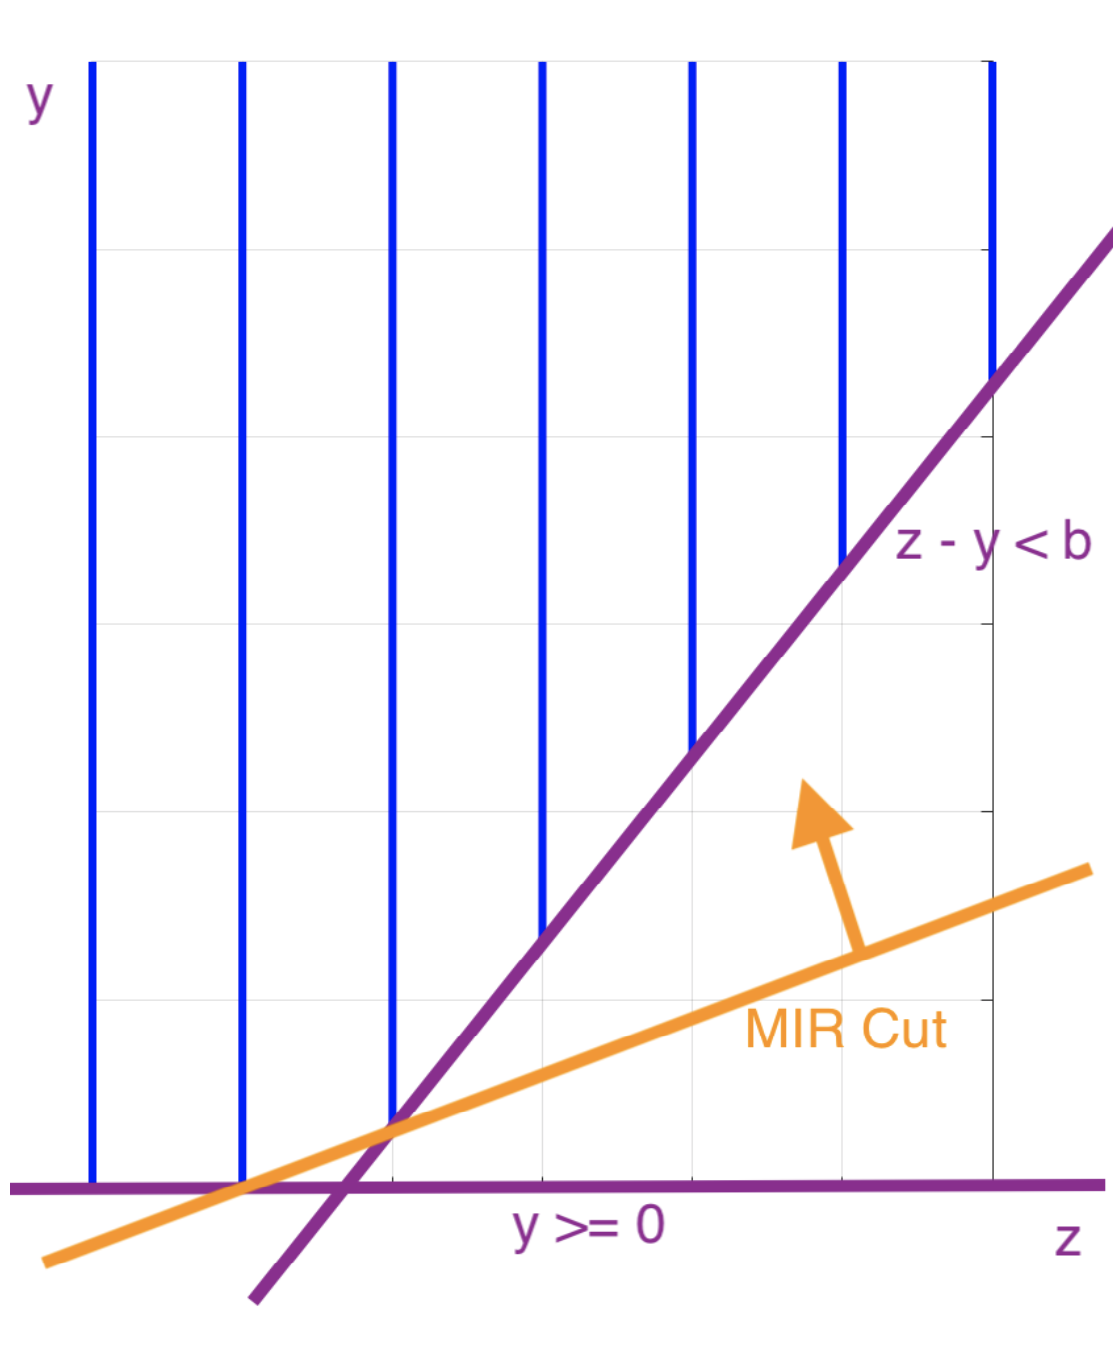
\includegraphics[scale = 0.3]{mir}
\end{center}
%\caption{Figure....}
%\end{figure}


\end{multicols}


\subsection{GMIC Derivation from MIR cut}
\begin{theorem}{Gomory Mixed Integer Cut - Pure Integer Case}{GMIC-Integer}
Suppose we have $x \in \Z^n_+$ with $x_i \in \Z$, along with the equation
\begin{equation}
\sum_{i \in I} a_{i}x_{i} = b.
\end{equation}
Then
\begin{equation}
\label{eq:gmic}
\sum_{i \in I^{-}} \frac{\{a_i\}}{f} x_i + \sum_{i \in I^+} \frac{1-\{a_i\}}{1-f}x_i \geq 1
\end{equation}
is valid for this set.
\end{theorem}


\begin{proof}
Let $I^- = \{ i \in I : \{a_i\} \leq f\}$, $I^+ = \{i \in I : \{a_i\}> f\}$.
\begin{equation}
\label{eq:tableau-gmic}
\sum_{i \in I^{-}} a_ix_i + \sum_{i \in I^+} a_i x_i = b
\end{equation}

Now we rewrite this as
\begin{equation}
\sum_{i \in I^{-}} (\floor{a_i} + \{a_i\} )x_i + \sum_{i \in I^+} (\ceil{a_i} - (1- \{a_i\})) x_i  = b
\end{equation}

Next, we remove fractional parts that are non-negative and keep ones that have negative coefficients.

\begin{equation}
\underbrace{\sum_{i \in I^{-}} \floor{a_i}x_i + \sum_{i \in I^+} \ceil{a_i}x_i }_{z} - \underbrace{\left( \sum_{i \in I^+}  (1- \{a_i\}) x_i \right)}_{y \geq 0} \leq b
\end{equation}

Applying the MIR cut, we obtain
\begin{equation}
\label{eq:gmic-mir}
\sum_{i \in I^{-}} \floor{a_i}x_i + \sum_{i \in I^+} \ceil{a_i}x_i - \sum_{i \in I^+}  \frac{1- \{a_i\}}{1-f} x_i \leq \floor{b}
\end{equation}

Now we subtract \eqref{eq:gmic-mir} from \eqref{eq:tableau-gmic} to obtain

\begin{equation}
\label{eq:gmic-close}
\sum_{i \in I^{-}} \underbrace{(a_i - \floor{a_i})}_{\{a_i\}}x_i + \sum_{i \in I^+} \underbrace{(a_i - \ceil{a_i})}_{\{a_i\} - 1}x_i + \sum_{i \in I^+}  \frac{1- \{a_i\}}{1-f} x_i \geq \underbrace{b - \floor{b}}_{f}
\end{equation}

Which rearranges to 

%\begin{equation}
%\label{eq:gmic-close2}
%\sum_{i \in I^{-}} \{a_i\} x_i + \sum_{i \in I^+} (\{a_i\} - 1)x_i + \sum_{i \in I^+}  \frac{1- \{a_i\}}{1-f} x_i + \sum_{i \in C^+} a_i x_i   + \sum_{i \in C^-} a_i x_i + \sum_{i \in C^-}\frac{a_i}{1-f} x_i  \geq f
%\end{equation}
%then we have

\begin{equation}
\label{eq:gmic-close2}
\sum_{i \in I^{-}} \{a_i\} x_i + \sum_{i \in I^+} (1-\{a_i\})\left(-1+\frac{1}{1-f}\right)x_i\geq f
\end{equation}

Lastly, we divide through by $f$.  Note that

\begin{equation*}
\frac{1}{f} \left(-1+\frac{1}{1-f}\right) = 
\frac{1}{f} \left(\frac{-(1-f) + 1}{1-f}\right) = 
\frac{1}{f} \left(\frac{f}{1-f}\right) = 
\frac{1}{1-f} 
\end{equation*}

Hence, we obtain

\begin{equation*}
\label{eq:gmic-end}
\sum_{i \in I^{-}} \frac{\{a_i\}}{f} x_i + \sum_{i \in I^+} \frac{1-\{a_i\}}{1-f}x_i  \geq 1
\end{equation*}


\end{proof}

\newpage
We now repeat the proof and show the mixed integer case to showcase the more general version.


\begin{theorem}{Gomory Mixed Integer Cut - Mixed integer case}{theoexample}
Suppose we have $x \in \R^n_+$ with $x_i \in \Z$ for all $ i \in I$, along with the equation
\begin{equation}
\sum_{i \in I} a_{i}x_{i} + \sum_{i \in C} a_{i}x_{i } = b.
\end{equation}
Then
\begin{equation}
\label{eq:gmic}
\sum_{i \in I^{-}} \frac{\{a_i\}}{f} x_i + \sum_{i \in I^+} \frac{1-\{a_i\}}{1-f}x_i + 
\sum_{i \in C^+} \frac{a_i}{f}\, x_i   + \sum_{i \in C^-}\frac{-a_i}{1-f}\,x_i \geq 1
\end{equation}
is valid for this set.
\end{theorem}


\begin{proof}
Let $I^- = \{ i \in I : \{a_i\} \leq f\}$, $I^+ = \{i \in I : \{a_i\}> f\}$ and let $C^-  = \{i \in C : a_i < 0\}$ and $C^+ = \{ i \in C : a_i \geq 0\}$.
\begin{equation*}
\label{eq:tableau-gmic}
\sum_{i \in I^{-}} a_ix_i + \sum_{i \in I^+} a_i x_i - \sum_{i \in C^-}(-a_i) x_i + \sum_{i \in C^+} a_i x_i = b
\end{equation*}

Now we rewrite this as
\begin{equation*}
\sum_{i \in I^{-}} (\floor{a_i} + \{a_i\} )x_i + \sum_{i \in I^+} (\ceil{a_i} - (1- \{a_i\})) x_i   - \sum_{i \in C^-}(-a_i) x_i + \sum_{i \in C^+} a_i x_i = b
\end{equation*}

Next, we remove fractional parts that are non-negative and keep ones that have negative coefficients.

\begin{equation}
\underbrace{\sum_{i \in I^{-}} \floor{a_i}x_i + \sum_{i \in I^+} \ceil{a_i}x_i }_{z} - \underbrace{\left( \sum_{i \in I^+}  (1- \{a_i\}) x_i   + \sum_{i \in C^-}(-a_i) x_i\right)}_{y \geq 0} \leq b
\end{equation}

Applying the MIR cut, we obtain
\begin{equation*}
\label{eq:gmic-mir}
\sum_{i \in I^{-}} \floor{a_i}x_i + \sum_{i \in I^+} \ceil{a_i}x_i - \sum_{i \in I^+}  \frac{1- \{a_i\}}{1-f} x_i   +  \sum_{i \in C^-}\frac{a_i}{1-f} x_i \leq \floor{b}
\end{equation*}

Now we subtract \eqref{eq:gmic-mir} from \eqref{eq:tableau-gmic} to obtain

\begin{equation*}
\label{eq:gmic-close}
\sum_{i \in I^{-}} \underbrace{(a_i - \floor{a_i})}_{\{a_i\}}x_i + \sum_{i \in I^+}\left( \underbrace{(a_i - \ceil{a_i})}_{\{a_i\} - 1}x_i +  \frac{1- \{a_i\}}{1-f} x_i   \right)+ \sum_{i \in C^+} a_i x_i + \sum_{i \in C^-} \left( a_i x_i +\frac{a_i}{1-f} x_i \right)\geq \underbrace{b - \floor{b}}_{f}
\end{equation*}

Which rearranges to 

%\begin{equation}
%\label{eq:gmic-close2}
%\sum_{i \in I^{-}} \{a_i\} x_i + \sum_{i \in I^+} (\{a_i\} - 1)x_i + \sum_{i \in I^+}  \frac{1- \{a_i\}}{1-f} x_i + \sum_{i \in C^+} a_i x_i   + \sum_{i \in C^-} a_i x_i + \sum_{i \in C^-}\frac{a_i}{1-f} x_i  \geq f
%\end{equation}
%then we have

\begin{equation}
\label{eq:gmic-close2}
\sum_{i \in I^{-}} \{a_i\} x_i + \sum_{i \in I^+} (1-\{a_i\})\left(-1+\frac{1}{1-f}\right)x_i + \sum_{i \in C^+} a_i x_i   + \sum_{i \in C^-}(-a_i)\left(-1 + \frac{1}{1-f}\right) x_i \geq f
\end{equation}

Lastly, we divide through by $f$.  Note that

\begin{equation*}
\frac{1}{f} \left(-1+\frac{1}{1-f}\right) = 
\frac{1}{f} \left(\frac{-(1-f) + 1}{1-f}\right) = 
\frac{1}{f} \left(\frac{f}{1-f}\right) = 
\frac{1}{1-f} 
\end{equation*}



Hence, we obtain

\begin{equation*}
\label{eq:gmic-end}
\sum_{i \in I^{-}} \frac{\{a_i\}}{f} x_i + \sum_{i \in I^+} \frac{1-\{a_i\}}{1-f}x_i + 
\sum_{i \in C^+} \frac{a_i}{f} x_i   + \sum_{i \in C^-}\frac{-a_i}{1-f}x_i \geq 1
\end{equation*}

\begin{equation*}
\label{eq:gmic-end}
\sum_{i \in I^{-}} \frac{\{a_i\}}{f} x_i + \sum_{i \in I^+} \frac{1-\{a_i\}}{1-f}x_i + 
\sum_{i \in C^+} \frac{a_i}{f} x_i   + \sum_{i \in C^-}\frac{-a_i}{1-f}x_i \geq 1
\end{equation*}
\end{proof}

If we let $\pi\colon \R \to \R_+$ map coefficients on integer variables to coefficients in the inequality and let $\psi \colon \R \to \R_+$ map coefficients on the continuous variables to coefficients on the inequalities, then these functions look like



\begin{figure}[h]
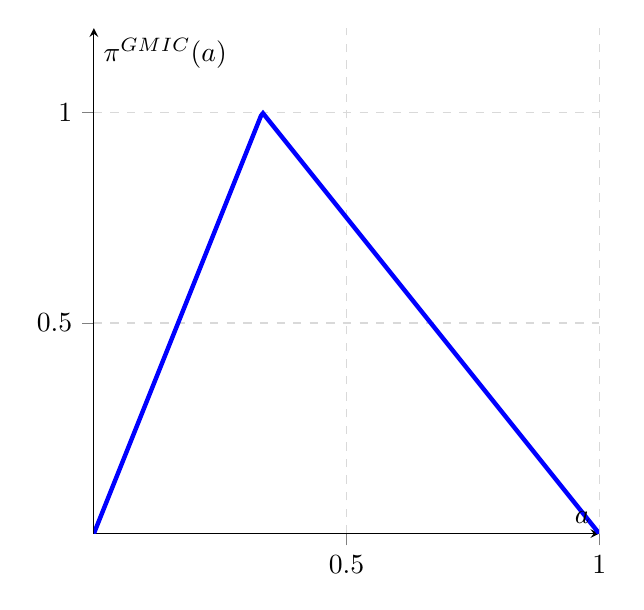
\begin{tikzpicture}
    \begin{axis}[
        axis x line=middle,
        axis y line=middle,
        grid = major,
        width=8cm,
        height=8cm,
        grid style={dashed, gray!30},
        xmin=0,     % start the diagram at this x-coordinate
        xmax= 1,    % end   the diagram at this x-coordinate
        ymin= 0,     % start the diagram at this y-coordinate
        ymax= 1.2,   % end   the diagram at this y-coordinate
        xlabel=$a$,
        ylabel=$\pi^\text{GMIC}(a)$,
		/pgfplots/xtick={-1, -0.5, ..., 1}, % make steps of length 0.5
		/pgfplots/ytick={0, 0.5, ..., 1}, % make steps of length 0.5
        tick align=outside,
        enlargelimits=false]
      % plot the function
	  \addplot[domain=-1:1, blue, ultra thick,samples=500] {x < 0.3333 ? 3*x : (x > 0.3333 ? 1.5-1.5*x  : x)};
    \end{axis}
\end{tikzpicture}
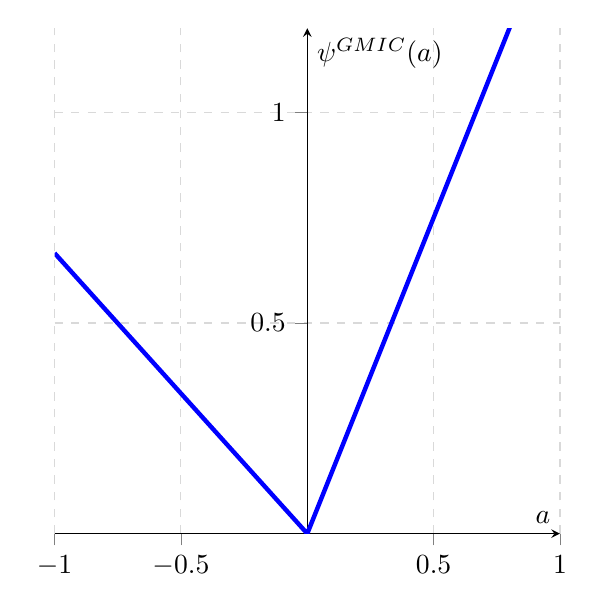
\begin{tikzpicture}
    \begin{axis}[
        axis x line=middle,
        axis y line=middle,
        grid = major,
        width=8cm,
        height=8cm,
        grid style={dashed, gray!30},
        xmin=-1,     % start the diagram at this x-coordinate
        xmax= 1,    % end   the diagram at this x-coordinate
        ymin= 0,     % start the diagram at this y-coordinate
        ymax= 1.2,   % end   the diagram at this y-coordinate
        xlabel=$a$,
        ylabel=$\psi^\text{GMIC}(a)$,
		/pgfplots/xtick={-1, -0.5, ..., 1}, % make steps of length 0.5
		/pgfplots/ytick={0, 0.5, ..., 1}, % make steps of length 0.5
        tick align=outside,
        enlargelimits=false]
      % plot the function
	  \addplot[domain=-1:1, blue, ultra thick,samples=500] {x < 0 ? -0.666*x : (x > 0 ? 1.5*x  : x)};
    \end{axis}
\end{tikzpicture}

\caption{Gomory mixed integer cut (GMIC) described by the pair of functions $(\pi, \psi)$ for $f = \tfrac{1}{3}$.}

\end{figure}



%\input{split_cuts_protected.tex}

\chapter{Dantzig Wolfe}

\begin{tabular}{cccccccccccccccccccccccccc}
       0  &       0  &       0  &       0  &       0  &       0  &       0  &       0  &       1  &       0  &       0  &       0  &       0  &       0  &       0  &       0  &       0  &       0  &       0  &       0  &       1  &       0  &       0  &       0 \\
       0  &       0  &       0  &       0  &       0  &       0  &       0  &       0  &       0  &       1  &       0  &       0  &       0  &       0  &       0  &       0  &       0  &       0  &       0  &       0  &       0  &       1  &       0  &       0 \\
       0  &       0  &       0  &       0  &       0  &       0  &       0  &       0  &       0  &       0  &       1  &       0  &       0  &       0  &       0  &       0  &       0  &       0  &       0  &       0  &       0  &       0  &       1  &       0 \\
       0  &       0  &       0  &       0  &       0  &       0  &       0  &       0  &       0  &       0  &       0  &       1  &       0  &       0  &       0  &       0  &       0  &       0  &       0  &       0  &       0  &       0  &       0  &       1 \\
       0  &       1  &       0  &       0  &       1  &     -1  &       0  &       0  &       0  &       0  &       0  &       0  &       0  &       0  &       0  &       0  &       0  &       0  &       0  &       0  &       0  &       0  &       0  &       0 \\
       0  &       0  &       1  &       0  &       0  &       1  &     -1  &       0  &       0  &       0  &       0  &       0  &       0  &       0  &       0  &       0  &       0  &       0  &       0  &       0  &       0  &       0  &       0  &       0 \\
       0  &       0  &       0  &       1  &       0  &       0  &       1  &     -1  &       0  &       0  &       0  &       0  &       0  &       0  &       0  &       0  &       0  &       0  &       0  &       0  &       0  &       0  &       0  &       0 \\
       1  &       0  &       0  &       0  &       0  &       0  &       0  &       0  &     -2  &       0  &       0  &       0  &       0  &       0  &       0  &       0  &       0  &       0  &       0  &       0  &       0  &       0  &       0  &       0 \\
       0  &       1  &       0  &       0  &       0  &       0  &       0  &       0  &       0  &     -3  &       0  &       0  &       0  &       0  &       0  &       0  &       0  &       0  &       0  &       0  &       0  &       0  &       0  &       0 \\
       0  &       0  &       1  &       0  &       0  &       0  &       0  &       0  &       0  &       0  &     -4  &       0  &       0  &       0  &       0  &       0  &       0  &       0  &       0  &       0  &       0  &       0  &       0  &       0 \\
       0  &       0  &       0  &       1  &       0  &       0  &       0  &       0  &       0  &       0  &       0  &     -5  &       0  &       0  &       0  &       0  &       0  &       0  &       0  &       0  &       0  &       0  &       0  &       0 \\
       0  &       0  &       0  &       0  &       0  &       0  &       0  &       0  &       0  &       0  &       0  &       0  &       0  &       1  &       0  &       0  &       1  &     -1  &       0  &       0  &       0  &       0  &       0  &       0 \\
       0  &       0  &       0  &       0  &       0  &       0  &       0  &       0  &       0  &       0  &       0  &       0  &       0  &       0  &       1  &       0  &       0  &       1  &     -1  &       0  &       0  &       0  &       0  &       0 \\
       0  &       0  &       0  &       0  &       0  &       0  &       0  &       0  &       0  &       0  &       0  &       0  &       0  &       0  &       0  &       1  &       0  &       0  &       1  &     -1  &       0  &       0  &       0  &       0 \\
       0  &       0  &       0  &       0  &       0  &       0  &       0  &       0  &       0  &       0  &       0  &       0  &       1  &       0  &       0  &       0  &       0  &       0  &       0  &       0  &     -4  &       0  &       0  &       0 \\
       0  &       0  &       0  &       0  &       0  &       0  &       0  &       0  &       0  &       0  &       0  &       0  &       0  &       1  &       0  &       0  &       0  &       0  &       0  &       0  &       0  &     -3  &       0  &       0 \\
       0  &       0  &       0  &       0  &       0  &       0  &       0  &       0  &       0  &       0  &       0  &       0  &       0  &       0  &       1  &       0  &       0  &       0  &       0  &       0  &       0  &       0  &     -1  &       0 \\
       0  &       0  &       0  &       0  &       0  &       0  &       0  &       0  &       0  &       0  &       0  &       0  &       0  &       0  &       0  &       1  &       0  &       0  &       0  &       0  &       0  &       0  &       0  &     -2 
\end{tabular}



\chapter{Lattices, IP in fixed dimensions}
A lattice is a rational linear transformation of the set of integer points.  That is, for a rational matrix $A \in \Q^{m \times n}$, the a lattice is the set $\Lambda = A\Z^n = \{x :  x = \sum_{i=1}^n a^i z_i, z \in \Z^n\}$ where $a^i$ are the columns of the matrix $A$.  
The dimension of the lattice $\Lambda$ is the dimension of the affine hull of $\Lambda$.  If $d = \dim(\aff(\Lambda))$, then there exists a rational matrix $A' \in \Q^{d\times n}$ such that $\Lambda = A'\Z^n$.  
For this reason, and the fact that we can project lattices into a more natural dimension, we typically assume that $A \in \Q^{n\times n}$ is invertible and that $\Lambda  = A\Z^n$ has dimension $n$.  \\
As mentioned in class, there are many possible choices of $A$ that describe the same lattice $\Lambda$.  The columns of $A$ are $n$-dimensional vectors that make up the lattice basis, and hence there are many choices of lattice bases.  \\
Here, is a lattice generated by the basis vectors $a^1= (3,1)$, $a^2 = (2,0)$.
\begin{center}
\begin{tikzpicture}
%\path[fill = gray] (0.25,0.25)--(0.25,3.75)--(3.75,3.75)--(3.75,0.25)--(0.25,0.25);
%\draw[help lines, color=gray!30, dashed] (0,0) grid (4.9,4.9);
%\draw[->,ultra thick] (0,0)--(5,0) node[right]{$x$};
%\draw[->,ultra thick] (0,0)--(0,5) node[above]{$y$};
%\foreach \x in {0,1,2,3,4}
    %\draw (\x cm,1pt) -- (\x cm,-1pt) node[anchor=north] {$\x$};
%\foreach \y in {0,1,2,3,4}
    %\draw (1pt,\y cm) -- (-1pt,\y cm) node[anchor=east] {$\y$};
\begin{scope}
\clip(-0.5,-0.5) rectangle (6.5,3.5);
\foreach \x in {0,1,2,3,4,5}
	\foreach \y in {0,1,2,3,4,5}
    		\filldraw (2*\x+\y-3,\y) circle (1.2pt);
\node (A) at (2,1) {};
\node (B) at (5,2) {};
\node (C) at (4,1) {};
\draw[thick,->] (A) -- (B) node[midway, above] {$a^1$};
\draw[thick,->] (A) -- (C) node[midway, below] {$a^2$};
\end{scope}
\end{tikzpicture}
\end{center}
The LLL algorithm, named for Lenstra, Lenstra, and Lovasz, is a polynomial time algorithm that uses Gram-Schmidt orthogonalization to take a basis matrix $A$ and make a better basis that is more orthogonal.  This makes various properties of the lattice easier to compute such as approximations to the shortest vector problem and the closest vector problem.  Some call the produced basis the LLL basis.   For Instance, the LLL algorithm reduces the above lattice basis to the new lattice basis $\bar a^1 = (1,1)$ and $\bar a^2 = (1,-1)$.   This scenario is ideal since the  basis vectors are orthogonal.
\begin{center}
\begin{tikzpicture}
\begin{scope}
\clip(-0.5,-0.5) rectangle (6.5,3.5);
\foreach \x in {0,1,2,3,4,5}
	\foreach \y in {0,1,2,3,4,5}
    		\filldraw (2*\x+\y-3,\y) circle (1.2pt);
\node (A) at (2,1) {};
\node (B) at (3,2) {};
\node (C) at (3,0) {};
\draw[thick,->] (A) -- (B) node[midway, above left] {$\bar a^1$};
\draw[thick,->] (A) -- (C) node[midway, below left] {$\bar a^2$};
\end{scope}
\end{tikzpicture}
\end{center}

 There are other bases such as the HKZ (or sometimes called the KZ) basis that is composed of the $n$-shortest vectors in the lattices (that is, the first vector in the basis the shortest vector, the second is the shortest vector in the lattice created by the last $n-1$ basis vectors, and so on).  This basis allows the computation of many problems exactly, but it takes exponential time to construct this basis.  There are also bases called BKZ (Block KZ) bases that for any fixed size of block $k$, it can be computed in polynomial time.  These bases interpolate between LLL and HKZ by if $k=1$, you get back LLL and if $k=n$ you obtain HKZ.\\
%\end{document}
